%----------------------
% S_4 Example
%----------------------
We dedicate a section to working through the case where $n=4.$
In this case, $\mathrm{S}_4(\calP) = \mathrm{S}_4\setminus\calP.$ So the permutations which do not correspond to squarefree monomial ideals (i.e., Stanley-Reisner ideals) are precisely those permutations in $\calP.$ 

 
We can check that the $v\in\calP$ produce simplicial complexes whose Stanley-Reisner ring is not the cohomology ring for $X_v$ by comparing the Hilbert series of the Stanley Reisner ring for $\Delta_v $ and the Poincar\'e polynomial for the corresponding Schubert variety $X_v.$ We do this explicitly in \Cref{tab:S4-bad-permutations} and demonstrate that the two polynomials disagree for all seven permutations in $\calP.$ One can check easily that these two polynomials agree for all seventeen permutations in $\mathrm{S}_4(\calP).$


\begin{table}[htbp]
\centering
\small
\renewcommand{\arraystretch}{1.8}
\begin{tabularx}{\textwidth}{
|>{\hsize=.50\hsize\centering\arraybackslash}X
|>{\hsize=.40\hsize\centering\arraybackslash}X
|>{\hsize=.45\hsize\centering\arraybackslash}X
|>{\hsize=.55\hsize\centering\arraybackslash}X
|>{\hsize=2.10\hsize\centering\arraybackslash}X
|>{\hsize=2.00\hsize\centering\arraybackslash}X
|}
\hline
\rowcolor{light-blue}
\raisebox{0.4em}{{\large $v$}}
& \raisebox{0.4em}{{\large $\ell(v)$}}
& \raisebox{0.4em}{{\large $A(v)$}}
& \raisebox{0.4em}{{\large $s_2v$}}
& \raisebox{0.4em}{{\large $\mathrm{Hilb}(R_{\Delta,n},t)$}}
& \raisebox{0.4em}{{\large $\mathrm{Poin}_{X_v}=\sum_{\omega\le v}t^{\ell(\omega)}$}}\rule{0pt}{2.2em}
\\
\hline
\rowcolor{grayish}
$2143$ & $2$ & $\{2\}$ & $3142$
& $1+3t+3t^2+t^3$
& $1+2t+t^2$ \\
\rowcolor{light-grayish}
$2341$ & $3$ & $\{2\}$ & $3241$
& $1+3t+4t^2+3t^3+t^4$
& $1+3t+3t^2+t^3$ \\
\rowcolor{grayish}
$2413$ & $3$ & $\{2\}$ & $3412$
& $1+3t+5t^2+4t^3+t^4$
& $1+3t+3t^2+t^3$ \\
\rowcolor{light-grayish}
$4123$ & $3$ & $\{2\}$ & $4132$
& $1+3t+4t^2+3t^3+t^4$
& $1+3t+3t^2+t^3$ \\
\rowcolor{grayish}
$2431$ & $4$ & $\{2\}$ & $3421$
& $1+3t+5t^2+5t^3+3t^4+t^5$
& $1+3t+4t^2+3t^3+t^4$ \\
\rowcolor{light-grayish}
$4213$ & $4$ & $\{2\}$ & $4312$
& $1+3t+5t^2+5t^3+3t^4+t^5$
& $1+3t+4t^2+3t^3+t^4$ \\
\rowcolor{grayish}
$4231$ & $5$ & $\{2\}$ & $4321$
& $1+3t+5t^2+6t^3+5t^4+3t^5+t^6$
& $1+3t+5t^2+6t^3+4t^4+t^5$ \\
\hline
\end{tabularx}
\caption{The seven permutations of $\calP\subset\mathrm{S}_4,$ i.e., those permutations in $\mathrm{S}_4$ outside of $\mathrm{S}_4(\calP)$.}
\label{tab:S4-bad-permutations}
\end{table}

The seven permutations in \Cref{tab:S4-bad-permutations} are exactly the $v\in\mathrm{S}_4$ with $A(v)\neq\varnothing.$ 
Here $i(v) = 1$ and $j(v) = 4.$ So, $[i+1,j-2] = \{2\}$ and $A(v) = \{2\}$ says the value $2$ precedes the value $3$ in $v,$ i.e., $v<s_2v.$ Thus in the fourth column, we look at $s_2v.$ Each of these are in $\mathrm{S}_4(\calP).$


In \Cref{fig: s4 simplicial complex poset}, we give the subposet of the (strong) Bruhat poset that corresponds to $\mathrm{S}_4(\calP)$ and we draw the simplicial complexes for each $w\in\mathrm{S}_4(\calP).$ The vertices in light gray represent those vertices that are singleton nonfaces. 

\begin{figure}[htbp]
    \centering
\begin{tikzpicture}[x=1cm, y=1cm,
  cell/.style={inner sep=2.5pt, outer sep=1.5pt},
  cov/.style={draw=black!40, line width=0.5pt}]
  \node[cell] (N1234) at (0.000,0.000) {\begin{tabular}{@{}c@{}}{\ttfamily\bfseries\small 1234}\\[0pt]%
\begin{tikzpicture}[scale=0.56, x=1cm, y=1cm,
  vtx/.style={circle, fill=black, inner sep=1.15pt},
  ghost/.style={circle, draw=black!30, fill=white, inner sep=1.0pt},
  ed/.style={line width=0.7pt, black!80}]
  \coordinate (v2) at (0.000,1.300);
  \coordinate (v3) at (-1.220,-0.780);
  \coordinate (v4) at (1.220,-0.780);
  \coordinate (v1) at (0.000,-0.060);
  \node[ghost] at (v1) {};
  \node[above right, black!35, inner sep=1.6pt, font=\scriptsize] at (v1) {$1$};
  \node[ghost] at (v2) {};
  \node[above, black!35, inner sep=1.6pt, font=\scriptsize] at (v2) {$2$};
  \node[ghost] at (v3) {};
  \node[below left, black!35, inner sep=1.6pt, font=\scriptsize] at (v3) {$3$};
  \node[ghost] at (v4) {};
  \node[below right, black!35, inner sep=1.6pt, font=\scriptsize] at (v4) {$4$};
\end{tikzpicture}\end{tabular}};
  \node[cell] (N1243) at (-3.350,2.980) {\begin{tabular}{@{}c@{}}{\ttfamily\bfseries\small 1243}\\[0pt]%
\begin{tikzpicture}[scale=0.56, x=1cm, y=1cm,
  vtx/.style={circle, fill=black, inner sep=1.15pt},
  ghost/.style={circle, draw=black!30, fill=white, inner sep=1.0pt},
  ed/.style={line width=0.7pt, black!80}]
  \coordinate (v2) at (0.000,1.300);
  \coordinate (v3) at (-1.220,-0.780);
  \coordinate (v4) at (1.220,-0.780);
  \coordinate (v1) at (0.000,-0.060);
  \node[ghost] at (v1) {};
  \node[above right, black!35, inner sep=1.6pt, font=\scriptsize] at (v1) {$1$};
  \node[ghost] at (v2) {};
  \node[above, black!35, inner sep=1.6pt, font=\scriptsize] at (v2) {$2$};
  \node[vtx] at (v3) {};
  \node[below left, inner sep=1.6pt, font=\scriptsize] at (v3) {$3$};
  \node[vtx] at (v4) {};
  \node[below right, inner sep=1.6pt, font=\scriptsize] at (v4) {$4$};
\end{tikzpicture}\end{tabular}};
  \node[cell] (N1324) at (0.000,2.980) {\begin{tabular}{@{}c@{}}{\ttfamily\bfseries\small 1324}\\[0pt]%
\begin{tikzpicture}[scale=0.56, x=1cm, y=1cm,
  vtx/.style={circle, fill=black, inner sep=1.15pt},
  ghost/.style={circle, draw=black!30, fill=white, inner sep=1.0pt},
  ed/.style={line width=0.7pt, black!80}]
  \coordinate (v2) at (0.000,1.300);
  \coordinate (v3) at (-1.220,-0.780);
  \coordinate (v4) at (1.220,-0.780);
  \coordinate (v1) at (0.000,-0.060);
  \node[ghost] at (v1) {};
  \node[above right, black!35, inner sep=1.6pt, font=\scriptsize] at (v1) {$1$};
  \node[vtx] at (v2) {};
  \node[above, inner sep=1.6pt, font=\scriptsize] at (v2) {$2$};
  \node[vtx] at (v3) {};
  \node[below left, inner sep=1.6pt, font=\scriptsize] at (v3) {$3$};
  \node[ghost] at (v4) {};
  \node[below right, black!35, inner sep=1.6pt, font=\scriptsize] at (v4) {$4$};
\end{tikzpicture}\end{tabular}};
  \node[cell] (N2134) at (3.350,2.980) {\begin{tabular}{@{}c@{}}{\ttfamily\bfseries\small 2134}\\[0pt]%
\begin{tikzpicture}[scale=0.56, x=1cm, y=1cm,
  vtx/.style={circle, fill=black, inner sep=1.15pt},
  ghost/.style={circle, draw=black!30, fill=white, inner sep=1.0pt},
  ed/.style={line width=0.7pt, black!80}]
  \coordinate (v2) at (0.000,1.300);
  \coordinate (v3) at (-1.220,-0.780);
  \coordinate (v4) at (1.220,-0.780);
  \coordinate (v1) at (0.000,-0.060);
  \node[vtx] at (v1) {};
  \node[above right, inner sep=1.6pt, font=\scriptsize] at (v1) {$1$};
  \node[vtx] at (v2) {};
  \node[above, inner sep=1.6pt, font=\scriptsize] at (v2) {$2$};
  \node[ghost] at (v3) {};
  \node[below left, black!35, inner sep=1.6pt, font=\scriptsize] at (v3) {$3$};
  \node[ghost] at (v4) {};
  \node[below right, black!35, inner sep=1.6pt, font=\scriptsize] at (v4) {$4$};
\end{tikzpicture}\end{tabular}};
  \node[cell] (N1342) at (-1.675,5.960) {\begin{tabular}{@{}c@{}}{\ttfamily\bfseries\small 1342}\\[0pt]%
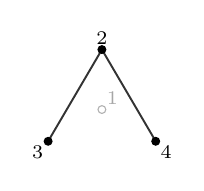
\begin{tikzpicture}[scale=0.56, x=1cm, y=1cm,
  vtx/.style={circle, fill=black, inner sep=1.15pt},
  ghost/.style={circle, draw=black!30, fill=white, inner sep=1.0pt},
  ed/.style={line width=0.7pt, black!80}]
  \coordinate (v2) at (0.000,1.300);
  \coordinate (v3) at (-1.220,-0.780);
  \coordinate (v4) at (1.220,-0.780);
  \coordinate (v1) at (0.000,-0.060);
  \draw[ed] (v2) -- (v3);
  \draw[ed] (v2) -- (v4);
  \node[ghost] at (v1) {};
  \node[above right, black!35, inner sep=1.6pt, font=\scriptsize] at (v1) {$1$};
  \node[vtx] at (v2) {};
  \node[above, inner sep=1.6pt, font=\scriptsize] at (v2) {$2$};
  \node[vtx] at (v3) {};
  \node[below left, inner sep=1.6pt, font=\scriptsize] at (v3) {$3$};
  \node[vtx] at (v4) {};
  \node[below right, inner sep=1.6pt, font=\scriptsize] at (v4) {$4$};
\end{tikzpicture}\end{tabular}};
  \node[cell] (N1423) at (-5.025,5.960) {\begin{tabular}{@{}c@{}}{\ttfamily\bfseries\small 1423}\\[0pt]%
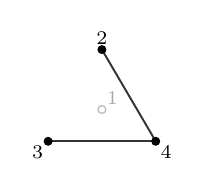
\begin{tikzpicture}[scale=0.56, x=1cm, y=1cm,
  vtx/.style={circle, fill=black, inner sep=1.15pt},
  ghost/.style={circle, draw=black!30, fill=white, inner sep=1.0pt},
  ed/.style={line width=0.7pt, black!80}]
  \coordinate (v2) at (0.000,1.300);
  \coordinate (v3) at (-1.220,-0.780);
  \coordinate (v4) at (1.220,-0.780);
  \coordinate (v1) at (0.000,-0.060);
  \draw[ed] (v2) -- (v4);
  \draw[ed] (v3) -- (v4);
  \node[ghost] at (v1) {};
  \node[above right, black!35, inner sep=1.6pt, font=\scriptsize] at (v1) {$1$};
  \node[vtx] at (v2) {};
  \node[above, inner sep=1.6pt, font=\scriptsize] at (v2) {$2$};
  \node[vtx] at (v3) {};
  \node[below left, inner sep=1.6pt, font=\scriptsize] at (v3) {$3$};
  \node[vtx] at (v4) {};
  \node[below right, inner sep=1.6pt, font=\scriptsize] at (v4) {$4$};
\end{tikzpicture}\end{tabular}};
  \node[cell] (N2314) at (5.025,5.960) {\begin{tabular}{@{}c@{}}{\ttfamily\bfseries\small 2314}\\[0pt]%
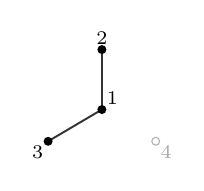
\begin{tikzpicture}[scale=0.56, x=1cm, y=1cm,
  vtx/.style={circle, fill=black, inner sep=1.15pt},
  ghost/.style={circle, draw=black!30, fill=white, inner sep=1.0pt},
  ed/.style={line width=0.7pt, black!80}]
  \coordinate (v2) at (0.000,1.300);
  \coordinate (v3) at (-1.220,-0.780);
  \coordinate (v4) at (1.220,-0.780);
  \coordinate (v1) at (0.000,-0.060);
  \draw[ed] (v1) -- (v2);
  \draw[ed] (v1) -- (v3);
  \node[vtx] at (v1) {};
  \node[above right, inner sep=1.6pt, font=\scriptsize] at (v1) {$1$};
  \node[vtx] at (v2) {};
  \node[above, inner sep=1.6pt, font=\scriptsize] at (v2) {$2$};
  \node[vtx] at (v3) {};
  \node[below left, inner sep=1.6pt, font=\scriptsize] at (v3) {$3$};
  \node[ghost] at (v4) {};
  \node[below right, black!35, inner sep=1.6pt, font=\scriptsize] at (v4) {$4$};
\end{tikzpicture}\end{tabular}};
  \node[cell] (N3124) at (1.675,5.960) {\begin{tabular}{@{}c@{}}{\ttfamily\bfseries\small 3124}\\[0pt]%
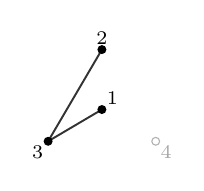
\begin{tikzpicture}[scale=0.56, x=1cm, y=1cm,
  vtx/.style={circle, fill=black, inner sep=1.15pt},
  ghost/.style={circle, draw=black!30, fill=white, inner sep=1.0pt},
  ed/.style={line width=0.7pt, black!80}]
  \coordinate (v2) at (0.000,1.300);
  \coordinate (v3) at (-1.220,-0.780);
  \coordinate (v4) at (1.220,-0.780);
  \coordinate (v1) at (0.000,-0.060);
  \draw[ed] (v1) -- (v3);
  \draw[ed] (v2) -- (v3);
  \node[vtx] at (v1) {};
  \node[above right, inner sep=1.6pt, font=\scriptsize] at (v1) {$1$};
  \node[vtx] at (v2) {};
  \node[above, inner sep=1.6pt, font=\scriptsize] at (v2) {$2$};
  \node[vtx] at (v3) {};
  \node[below left, inner sep=1.6pt, font=\scriptsize] at (v3) {$3$};
  \node[ghost] at (v4) {};
  \node[below right, black!35, inner sep=1.6pt, font=\scriptsize] at (v4) {$4$};
\end{tikzpicture}\end{tabular}};
  \node[cell] (N1432) at (-3.350,8.940) {\begin{tabular}{@{}c@{}}{\ttfamily\bfseries\small 1432}\\[0pt]%
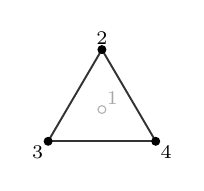
\begin{tikzpicture}[scale=0.56, x=1cm, y=1cm,
  vtx/.style={circle, fill=black, inner sep=1.15pt},
  ghost/.style={circle, draw=black!30, fill=white, inner sep=1.0pt},
  ed/.style={line width=0.7pt, black!80}]
  \coordinate (v2) at (0.000,1.300);
  \coordinate (v3) at (-1.220,-0.780);
  \coordinate (v4) at (1.220,-0.780);
  \coordinate (v1) at (0.000,-0.060);
  \draw[ed] (v2) -- (v3);
  \draw[ed] (v2) -- (v4);
  \draw[ed] (v3) -- (v4);
  \node[ghost] at (v1) {};
  \node[above right, black!35, inner sep=1.6pt, font=\scriptsize] at (v1) {$1$};
  \node[vtx] at (v2) {};
  \node[above, inner sep=1.6pt, font=\scriptsize] at (v2) {$2$};
  \node[vtx] at (v3) {};
  \node[below left, inner sep=1.6pt, font=\scriptsize] at (v3) {$3$};
  \node[vtx] at (v4) {};
  \node[below right, inner sep=1.6pt, font=\scriptsize] at (v4) {$4$};
\end{tikzpicture}\end{tabular}};
  \node[cell] (N3142) at (0.000,8.940) {\begin{tabular}{@{}c@{}}{\ttfamily\bfseries\small 3142}\\[0pt]%
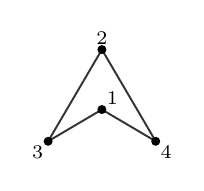
\begin{tikzpicture}[scale=0.56, x=1cm, y=1cm,
  vtx/.style={circle, fill=black, inner sep=1.15pt},
  ghost/.style={circle, draw=black!30, fill=white, inner sep=1.0pt},
  ed/.style={line width=0.7pt, black!80}]
  \coordinate (v2) at (0.000,1.300);
  \coordinate (v3) at (-1.220,-0.780);
  \coordinate (v4) at (1.220,-0.780);
  \coordinate (v1) at (0.000,-0.060);
  \draw[ed] (v1) -- (v3);
  \draw[ed] (v1) -- (v4);
  \draw[ed] (v2) -- (v3);
  \draw[ed] (v2) -- (v4);
  \node[vtx] at (v1) {};
  \node[above right, inner sep=1.6pt, font=\scriptsize] at (v1) {$1$};
  \node[vtx] at (v2) {};
  \node[above, inner sep=1.6pt, font=\scriptsize] at (v2) {$2$};
  \node[vtx] at (v3) {};
  \node[below left, inner sep=1.6pt, font=\scriptsize] at (v3) {$3$};
  \node[vtx] at (v4) {};
  \node[below right, inner sep=1.6pt, font=\scriptsize] at (v4) {$4$};
\end{tikzpicture}\end{tabular}};
  \node[cell] (N3214) at (3.350,8.940) {\begin{tabular}{@{}c@{}}{\ttfamily\bfseries\small 3214}\\[0pt]%
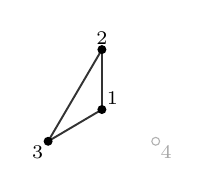
\begin{tikzpicture}[scale=0.56, x=1cm, y=1cm,
  vtx/.style={circle, fill=black, inner sep=1.15pt},
  ghost/.style={circle, draw=black!30, fill=white, inner sep=1.0pt},
  ed/.style={line width=0.7pt, black!80}]
  \coordinate (v2) at (0.000,1.300);
  \coordinate (v3) at (-1.220,-0.780);
  \coordinate (v4) at (1.220,-0.780);
  \coordinate (v1) at (0.000,-0.060);
  \draw[ed] (v1) -- (v2);
  \draw[ed] (v1) -- (v3);
  \draw[ed] (v2) -- (v3);
  \node[vtx] at (v1) {};
  \node[above right, inner sep=1.6pt, font=\scriptsize] at (v1) {$1$};
  \node[vtx] at (v2) {};
  \node[above, inner sep=1.6pt, font=\scriptsize] at (v2) {$2$};
  \node[vtx] at (v3) {};
  \node[below left, inner sep=1.6pt, font=\scriptsize] at (v3) {$3$};
  \node[ghost] at (v4) {};
  \node[below right, black!35, inner sep=1.6pt, font=\scriptsize] at (v4) {$4$};
\end{tikzpicture}\end{tabular}};
  \node[cell] (N3241) at (3.350,11.920) {\begin{tabular}{@{}c@{}}{\ttfamily\bfseries\small 3241}\\[0pt]%
\begin{tikzpicture}[scale=0.56, x=1cm, y=1cm,
  vtx/.style={circle, fill=black, inner sep=1.15pt},
  ghost/.style={circle, draw=black!30, fill=white, inner sep=1.0pt},
  ed/.style={line width=0.7pt, black!80}]
  \coordinate (v2) at (0.000,1.300);
  \coordinate (v3) at (-1.220,-0.780);
  \coordinate (v4) at (1.220,-0.780);
  \coordinate (v1) at (0.000,-0.060);
  \fill[faceblue] (v1) -- (v2) -- (v3) -- cycle;
  \fill[faceblue] (v1) -- (v2) -- (v4) -- cycle;
  \draw[ed] (v1) -- (v2);
  \draw[ed] (v1) -- (v3);
  \draw[ed] (v1) -- (v4);
  \draw[ed] (v2) -- (v3);
  \draw[ed] (v2) -- (v4);
  \node[vtx] at (v1) {};
  \node[above right, inner sep=1.6pt, font=\scriptsize] at (v1) {$1$};
  \node[vtx] at (v2) {};
  \node[above, inner sep=1.6pt, font=\scriptsize] at (v2) {$2$};
  \node[vtx] at (v3) {};
  \node[below left, inner sep=1.6pt, font=\scriptsize] at (v3) {$3$};
  \node[vtx] at (v4) {};
  \node[below right, inner sep=1.6pt, font=\scriptsize] at (v4) {$4$};
\end{tikzpicture}\end{tabular}};
  \node[cell] (N3412) at (0.000,11.920) {\begin{tabular}{@{}c@{}}{\ttfamily\bfseries\small 3412}\\[0pt]%
\begin{tikzpicture}[scale=0.56, x=1cm, y=1cm,
  vtx/.style={circle, fill=black, inner sep=1.15pt},
  ghost/.style={circle, draw=black!30, fill=white, inner sep=1.0pt},
  ed/.style={line width=0.7pt, black!80}]
  \coordinate (v2) at (0.000,1.300);
  \coordinate (v3) at (-1.220,-0.780);
  \coordinate (v4) at (1.220,-0.780);
  \coordinate (v1) at (0.000,-0.060);
  \fill[faceblue] (v1) -- (v2) -- (v4) -- cycle;
  \fill[faceblue] (v1) -- (v3) -- (v4) -- cycle;
  \draw[ed] (v1) -- (v2);
  \draw[ed] (v1) -- (v3);
  \draw[ed] (v1) -- (v4);
  \draw[ed] (v2) -- (v3);
  \draw[ed] (v2) -- (v4);
  \draw[ed] (v3) -- (v4);
  \node[vtx] at (v1) {};
  \node[above right, inner sep=1.6pt, font=\scriptsize] at (v1) {$1$};
  \node[vtx] at (v2) {};
  \node[above, inner sep=1.6pt, font=\scriptsize] at (v2) {$2$};
  \node[vtx] at (v3) {};
  \node[below left, inner sep=1.6pt, font=\scriptsize] at (v3) {$3$};
  \node[vtx] at (v4) {};
  \node[below right, inner sep=1.6pt, font=\scriptsize] at (v4) {$4$};
\end{tikzpicture}\end{tabular}};
  \node[cell] (N4132) at (-3.350,11.920) {\begin{tabular}{@{}c@{}}{\ttfamily\bfseries\small 4132}\\[0pt]%
\begin{tikzpicture}[scale=0.56, x=1cm, y=1cm,
  vtx/.style={circle, fill=black, inner sep=1.15pt},
  ghost/.style={circle, draw=black!30, fill=white, inner sep=1.0pt},
  ed/.style={line width=0.7pt, black!80}]
  \coordinate (v2) at (0.000,1.300);
  \coordinate (v3) at (-1.220,-0.780);
  \coordinate (v4) at (1.220,-0.780);
  \coordinate (v1) at (0.000,-0.060);
  \fill[faceblue] (v1) -- (v3) -- (v4) -- cycle;
  \draw[ed, dashed] (v1) -- (v3);
  \draw[ed, dashed] (v1) -- (v4);
  \draw[ed] (v2) -- (v3);
  \draw[ed] (v2) -- (v4);
  \draw[ed] (v3) -- (v4);
  \node[vtx] at (v1) {};
  \node[above right, inner sep=1.6pt, font=\scriptsize] at (v1) {$1$};
  \node[vtx] at (v2) {};
  \node[above, inner sep=1.6pt, font=\scriptsize] at (v2) {$2$};
  \node[vtx] at (v3) {};
  \node[below left, inner sep=1.6pt, font=\scriptsize] at (v3) {$3$};
  \node[vtx] at (v4) {};
  \node[below right, inner sep=1.6pt, font=\scriptsize] at (v4) {$4$};
\end{tikzpicture}\end{tabular}};
  \node[cell] (N3421) at (1.675,14.900) {\begin{tabular}{@{}c@{}}{\ttfamily\bfseries\small 3421}\\[0pt]%
\begin{tikzpicture}[scale=0.56, x=1cm, y=1cm,
  vtx/.style={circle, fill=black, inner sep=1.15pt},
  ghost/.style={circle, draw=black!30, fill=white, inner sep=1.0pt},
  ed/.style={line width=0.7pt, black!80}]
  \coordinate (v2) at (0.000,1.300);
  \coordinate (v3) at (-1.220,-0.780);
  \coordinate (v4) at (1.220,-0.780);
  \coordinate (v1) at (0.000,-0.060);
  \fill[faceblue] (v1) -- (v2) -- (v3) -- cycle;
  \fill[faceblue] (v1) -- (v2) -- (v4) -- cycle;
  \fill[faceblue] (v1) -- (v3) -- (v4) -- cycle;
  \draw[ed] (v1) -- (v2);
  \draw[ed] (v1) -- (v3);
  \draw[ed] (v1) -- (v4);
  \draw[ed] (v2) -- (v3);
  \draw[ed] (v2) -- (v4);
  \draw[ed] (v3) -- (v4);
  \node[vtx] at (v1) {};
  \node[above right, inner sep=1.6pt, font=\scriptsize] at (v1) {$1$};
  \node[vtx] at (v2) {};
  \node[above, inner sep=1.6pt, font=\scriptsize] at (v2) {$2$};
  \node[vtx] at (v3) {};
  \node[below left, inner sep=1.6pt, font=\scriptsize] at (v3) {$3$};
  \node[vtx] at (v4) {};
  \node[below right, inner sep=1.6pt, font=\scriptsize] at (v4) {$4$};
\end{tikzpicture}\end{tabular}};
  \node[cell] (N4312) at (-1.675,14.900) {\begin{tabular}{@{}c@{}}{\ttfamily\bfseries\small 4312}\\[0pt]%
\begin{tikzpicture}[scale=0.56, x=1cm, y=1cm,
  vtx/.style={circle, fill=black, inner sep=1.15pt},
  ghost/.style={circle, draw=black!30, fill=white, inner sep=1.0pt},
  ed/.style={line width=0.7pt, black!80}]
  \coordinate (v2) at (0.000,1.300);
  \coordinate (v3) at (-1.220,-0.780);
  \coordinate (v4) at (1.220,-0.780);
  \coordinate (v1) at (0.000,-0.060);
  \fill[faceblue] (v1) -- (v2) -- (v4) -- cycle;
  \fill[faceblue] (v1) -- (v3) -- (v4) -- cycle;
  \draw[ed, dashed] (v1) -- (v2);
  \draw[ed, dashed] (v1) -- (v3);
  \draw[ed, dashed] (v1) -- (v4);
  \draw[ed] (v2) -- (v3);
  \draw[ed] (v2) -- (v4);
  \draw[ed] (v3) -- (v4);
  \node[vtx] at (v1) {};
  \node[above right, inner sep=1.6pt, font=\scriptsize] at (v1) {$1$};
  \node[vtx] at (v2) {};
  \node[above, inner sep=1.6pt, font=\scriptsize] at (v2) {$2$};
  \node[vtx] at (v3) {};
  \node[below left, inner sep=1.6pt, font=\scriptsize] at (v3) {$3$};
  \node[vtx] at (v4) {};
  \node[below right, inner sep=1.6pt, font=\scriptsize] at (v4) {$4$};
\end{tikzpicture}\end{tabular}};
  \node[cell] (N4321) at (0.000,17.880) {\begin{tabular}{@{}c@{}}{\ttfamily\bfseries\small 4321}\\[0pt]%
\begin{tikzpicture}[scale=0.56, x=1cm, y=1cm,
  vtx/.style={circle, fill=black, inner sep=1.15pt},
  ghost/.style={circle, draw=black!30, fill=white, inner sep=1.0pt},
  ed/.style={line width=0.7pt, black!80}]
  \coordinate (v2) at (0.000,1.300);
  \coordinate (v3) at (-1.220,-0.780);
  \coordinate (v4) at (1.220,-0.780);
  \coordinate (v1) at (0.000,-0.060);
  \fill[faceblue] (v1) -- (v2) -- (v3) -- cycle;
  \fill[faceblue] (v1) -- (v2) -- (v4) -- cycle;
  \fill[faceblue] (v1) -- (v3) -- (v4) -- cycle;
  \draw[ed, dashed] (v1) -- (v2);
  \draw[ed, dashed] (v1) -- (v3);
  \draw[ed, dashed] (v1) -- (v4);
  \draw[ed] (v2) -- (v3);
  \draw[ed] (v2) -- (v4);
  \draw[ed] (v3) -- (v4);
  \node[vtx] at (v1) {};
  \node[above right, inner sep=1.6pt, font=\scriptsize] at (v1) {$1$};
  \node[vtx] at (v2) {};
  \node[above, inner sep=1.6pt, font=\scriptsize] at (v2) {$2$};
  \node[vtx] at (v3) {};
  \node[below left, inner sep=1.6pt, font=\scriptsize] at (v3) {$3$};
  \node[vtx] at (v4) {};
  \node[below right, inner sep=1.6pt, font=\scriptsize] at (v4) {$4$};
\end{tikzpicture}\end{tabular}};
  \draw[cov] (N1234) -- (N1243);
  \draw[cov] (N1234) -- (N1324);
  \draw[cov] (N1243) -- (N1342);
  \draw[cov] (N1324) -- (N1342);
  \draw[cov] (N1243) -- (N1423);
  \draw[cov] (N1324) -- (N1423);
  \draw[cov] (N1342) -- (N1432);
  \draw[cov] (N1423) -- (N1432);
  \draw[cov] (N1234) -- (N2134);
  \draw[cov] (N1324) -- (N2314);
  \draw[cov] (N2134) -- (N2314);
  \draw[cov] (N1324) -- (N3124);
  \draw[cov] (N2134) -- (N3124);
  \draw[cov] (N1342) -- (N3142);
  \draw[cov] (N3124) -- (N3142);
  \draw[cov] (N2314) -- (N3214);
  \draw[cov] (N3124) -- (N3214);
  \draw[cov] (N3142) -- (N3241);
  \draw[cov] (N3214) -- (N3241);
  \draw[cov] (N1432) -- (N3412);
  \draw[cov] (N3142) -- (N3412);
  \draw[cov] (N3214) -- (N3412);
  \draw[cov] (N3241) -- (N3421);
  \draw[cov] (N3412) -- (N3421);
  \draw[cov] (N1432) -- (N4132);
  \draw[cov] (N3142) -- (N4132);
  \draw[cov] (N3412) -- (N4312);
  \draw[cov] (N4132) -- (N4312);
  \draw[cov] (N3421) -- (N4321);
  \draw[cov] (N4312) -- (N4321);
\end{tikzpicture}
    \caption{The subposet of $\mathrm{S}_4$ given by $w\in\mathrm{S}_4(\calP)$ and the corresponding simplicial complexes $\Delta_w.$}
    \label{fig: s4 simplicial complex poset}
\end{figure}